\section{Experimental Evaluation}
\label{sec:exp_belief}

In this section, we evaluate the empirical performance of our belief representation network for different tasks, in deterministic or stochastic environments. 
In \Cref{subsec:setting_exp_belief}, we describe the setting of each task, of the baselines, and of D-TRPO. 
In \Cref{subsec:results_belief}, we provide and discuss the results of the experiments.

\subsection{Setting}
\label{subsec:setting_exp_belief}

Note that all the results for all the baselines, for our approach, and for all the tasks are averaged over 10 seeds.

\subsubsection{Tasks}
\label{subsubsec:tasks}
\noindent\textbf{Pendulum.}\indent In this task, the agent must learn to rotate a pendulum upward. 
This task is classic in delayed \gls{rl} because the performance of traditional \gls{rl} algorithms drops rapidly as the delay increases. 
This is in part due to the unstable equilibrium in the upward position, which is difficult to maintain when delayed. 
In the implementation, we use the version of the \texttt{gym} library~\cite{brockman2016gym}.
This environment is deterministic. 
Given the relatively low computational cost of running experiments on the Pendulum, we repeat the analysis for constant delays in the set $\{3, 5, 10, 15, 20\}$.
For this task, we performed 500 epochs of 5,000 steps each, for a total of 2.5 million steps.

\noindent\textbf{Stochastic Pendulum.}\indent This task is simply the same as the previous one, but stochasticity is artificially added to the process. 
To do so, we add an i.i.d. noise of the form $\epsilon = \text{scale}( \eta+ \text{shift})$ to the action selected by the agent, where $\eta$ is some probability distribution.
The six noises considered are given in \Cref{tab:noises}. 
An additional noise is considered, where the environment follows the action indicated by the agent with a probability of 0.9 but otherwise samples an action uniformly at random. 
We call this process the \emph{uniform} noise.
For these tasks, we consider only a delay of 5, we perform 1000 epochs of 5,000 steps each, for a total of 5 million steps.

\begin{table}[t]
\centering
    \begin{tabular}{|l||l|l|l|l|}
        \hline
        Noise & Distribution  $\eta$ & Shift & Scale & Group \\ \hline
        \textit{Beta (8,2)}& $\beta (8,2)$ & $0.5$ & $2$ &  1\\ 
        \textit{Beta (2,2)} & $\beta (2,2)$ & $0.5$ & $2$ & 1\\ 
        \textit{U-Shaped} & $\beta (0.5,0.5)$ & $0.5$ & $2$ & 1\\ 
        \textit{Triangular} & $\text{Triangular} (-2,1,2)$ & $0$ & $1$ & 2\\ 
        % \textit{Uniform} & $\text{U} (-1,1)$ & $0$ & $1$ & 2\\ 
        \textit{Lognormal (1)} & $\text{Lognormal} (0,1)$ & $-1$ & $1$ & 3\\ 
        \textit{Lognormal (0.1)} & $\text{Lognormal} (0,0.1)$ & $-1$ & $1$ & 3\\ 
        \hline
    \end{tabular}
    \caption{Distributions for the noise added to the action in the stochastic Pendulum.}
    \label{tab:noises}
\end{table}

\noindent\textbf{Mujoco.}\indent This is a continuous robotic locomotion control task where an advanced physics simulator is used, provided by the library \texttt{mujoco}~\cite{todorov2012mujoco}. 
The complexity of these tasks lies in their intricate dynamics and in the large state and action spaces. 
From all Mujoco environments, we consider Walker2d, HalfCheetah, Reacher, and Swimmer which, after early testing, were shown to be the most affected by the delay.
Similarly to the Pendulum, this can be explained by the presence of an unstable equilibrium in some cases. 
These environments are deterministic. 
For these tasks, we consider only a delay of 5, and perform 1,000 epochs of 5,000 steps each, for a total of 5 million steps.


\subsubsection{Baselines}
\label{subsubsec:baselines}
As baselines, we include \gls{trpo} with the augmented state (A-TRPO) and memoryless \gls{trpo} (M-TRPO) to have a spectrum of approaches based on \gls{trpo}. 
In addition, we consider \gls{sac} for the great empirical results that it has obtained when applied to delay\cite{ramstedt2019real,bouteiller2020reinforcement}. 
We also include \gls{sac} with an augmented state (A-SAC) and \gls{sac} with a memoryless state (M-SAC) in our baselines.
A hyperparameter for \gls{sac} is the frequency at which it is updated.
Although setting this parameter to retrain at each step increases sample efficiency, it drastically increases the computational time and memory usage. 
For this reason, we trained \gls{sac} at every step for Pendulum only, while restricting the training to every 50 steps on Mujoco to speed up the procedure.
We considered adding DCAC~\cite{bouteiller2020reinforcement} but its implementation happened to be computationally expensive, and we decided not to include it. 
Early experimental results showed that its run time was more than 10 times that of the other algorithms. 
Furthermore, we consider SARSA and dSARSA with $\lambda=0.9$ but only for the Pendulum environment. Since SARSA is a batch \gls{rl} algorithm, it requires careful discretisation of the state and action spaces, which has a direct impact on the final performance. 
Therefore, it requires an additional step of validation of the discretisation. 
For the Pendulum, we used a tuned 15x15 grid for the state space and a total of five discrete actions.
Lastly, we include L2-TRPO as a baseline in our tests, as it learns the expected value of the state using a similar approach to \cite{firoiu2018human}.


\subsubsection{Setting for D-TRPO}
In the experiments presented here, we test D-TRPO which results from plugging our belief representation network into \gls{trpo}~\cite{schulman2015trust}.
An important remark is that, after early experiments with D-TRPO, we have noted that the belief representation can change significantly as the belief module is being optimised.
In turn, this implies an unstable optimisation of the policy of \gls{trpo}, since its input distribution is constantly changing. 
To alleviate this problem, we propose the early stopping of the training of the belief representation module after 200 epochs. 


\subsection{Results}
\label{subsec:results_belief}

\begin{figure}[t]
    \centering
    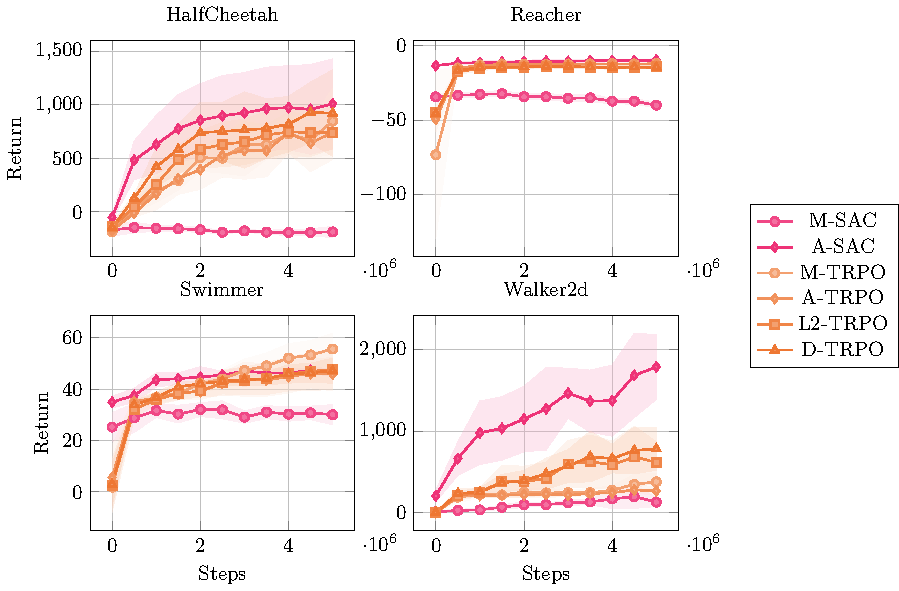
\includegraphics[labelbelief=pendulumvaryingdelay]{img/thesis_plots_belief.pdf}
    \caption{Mean return of D-TRPO and baselines for the Pendulum environment for different values of the delay. 
    The horizontal dashed line indicates undelayed \gls{sac}'s performance. 
    Shaded areas represent one standard deviation and the results are obtained for 10 seeds.}
    \label{fig:pendulum_varying_delay_belief}
\end{figure}

\noindent\textbf{Pendulum.}\indent The returns for the different approaches and for different values of the delay are provided in \Cref{fig:pendulum_varying_delay_imitation}. 
The horizontal dashed line indicates the return obtained by an undelayed version of \gls{sac}. 
For delays of up to five, D-TRPO and L2-TRPO have a return comparable to that of the undelayed \gls{sac}.
Note also the great performance of A-SAC in this case.
However, as the delay increases, the performance of D-TRPO and L2-TRPO drops more significantly than that of A-SAC.
In \Cref{fig:delay_5_pendulum_belief}, we focus on the performance of D-TRPO and the baselines for a delay of 5 during the learning phase. 
In the figure, we also report the result for undelayed \gls{trpo}. Naturally, the latter is faster than any delayed approach with \gls{trpo} but interestingly, it is slower than A-SAC. 
This suggests that SAC is particularly efficient in addressing this problem, even in the presence of delays.
Apart from A-SAC, D-TRPO and L2-TRPO have the fastest convergence rates and require around 1 million extra steps compared to undelayed TRPO to reach a similar policy.



\begin{figure}[t]
    \centering
    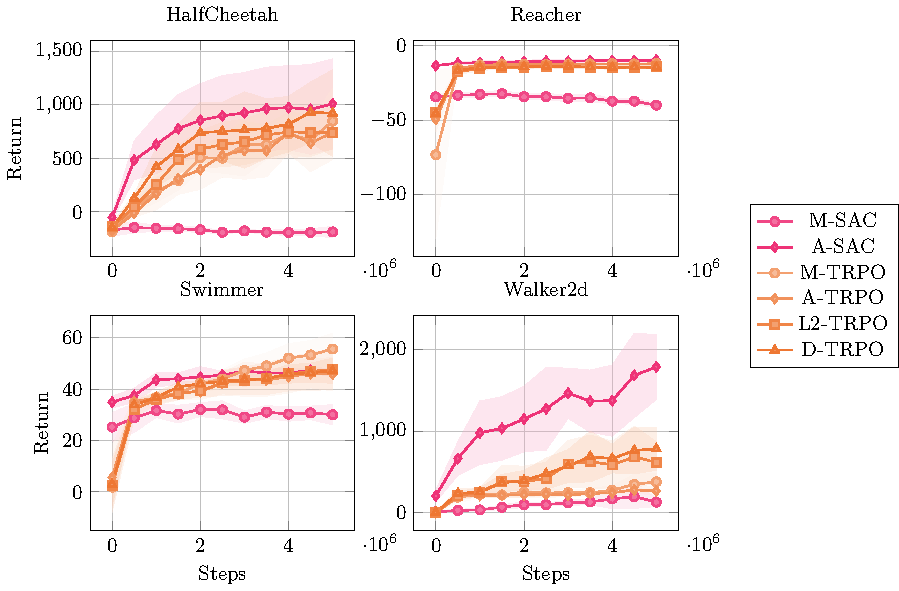
\includegraphics[labelbelief=delay5pendulumbelief]{img/thesis_plots_belief.pdf}
    \caption{Return obtained by D-TRPO and L2-TRPO compared to other baselines for the Pendulum task with delay 5. Undelayed \gls{trpo}'s performance, referred to as ``TRPO'', is included for comparison.
    Shaded areas represent one standard deviation and the results are obtained for 10 seeds.}
    \label{fig:delay_5_pendulum_belief}
\end{figure}

\noindent\textbf{Mujoco.}\indent In \Cref{fig:delay_5_mujoco_belief}, we report the results for the mujoco environments. 
Here as well, A-SAC is particularly efficient, not coming as first for only the Swimmer environment. 
Surprisingly, it is M-TRPO that performs best in this environment after 5 million steps. 
D-TRPO and L2-TRPO perform well in all environments, showing significant underperformance for Walker2d only.

\begin{figure}[t]
    \centering
    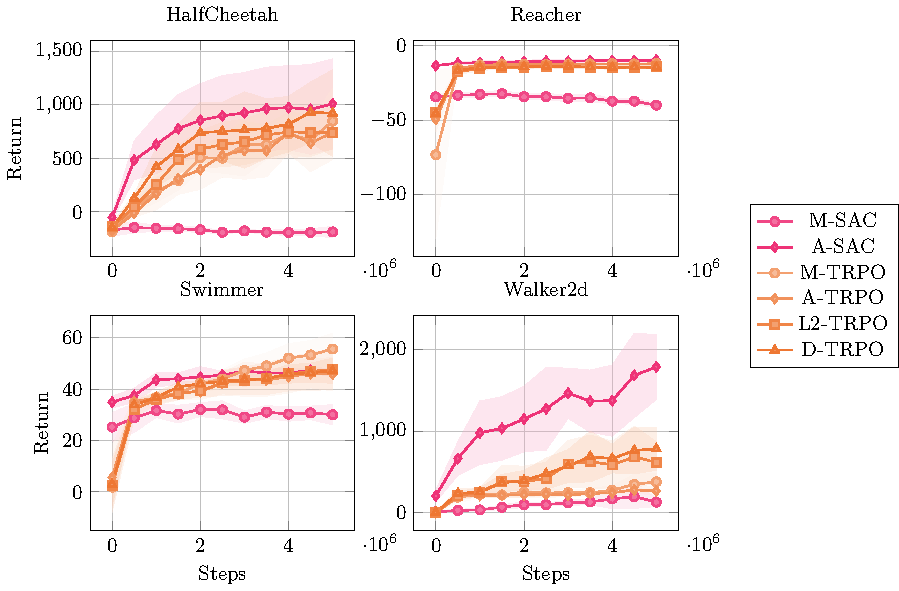
\includegraphics[labelbelief=delayfivemujocobelief]{img/thesis_plots_belief.pdf}
    \caption{Return obtained by D-TRPO and L2-TRPO compared to baselines for various Mujoco environments.
    Shaded area indicate one standard deviation and the results are obtained for 10 seeds.}
    \label{fig:delay_5_mujoco_belief}
\end{figure}

\noindent\textbf{Stochastic Pendulum.}\indent On this task, we solely compare D-TRPO with L2-TRPO, to evaluate the advantage of learning a representation of the belief of a future state over its mean. 
We report the results in \Cref{fig:delay_5_pendulum_noise_belief}. 
For the readability of the results, we have grouped the noise into 3 groups.
One can observe that D-TRPO is never outperformed by L2-TRPO. 
For some of the noises, they obtain similar performances, such as for Uniform and Triangular noises.
Yet, for other types of noise, the difference in performance is clearer, as for the Quadratic and LogNormal (0.1) cases. 
This suggests that the belief representation is at worst unnecessary, but at best it provides higher performance. 

\begin{figure}[t]
    \centering
    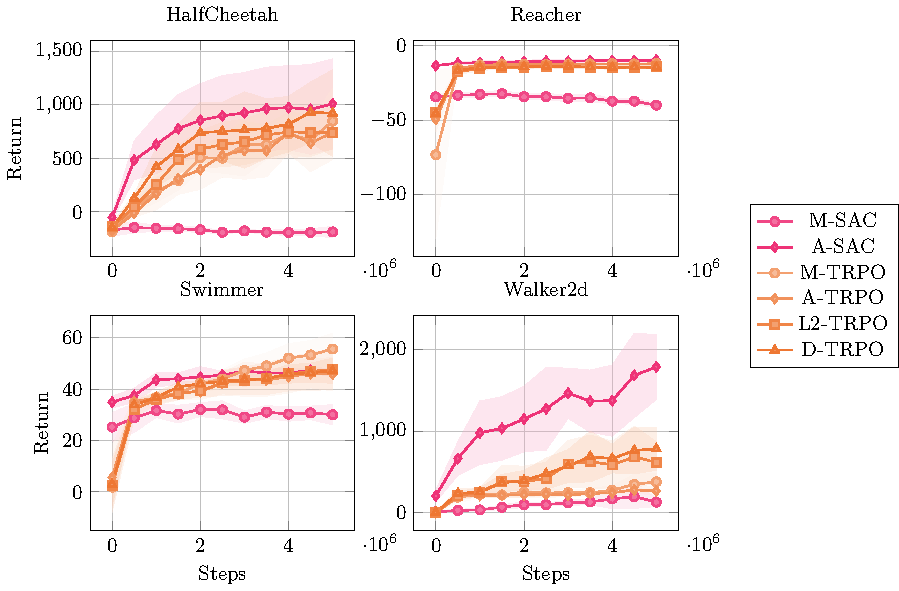
\includegraphics[labelbelief=pendulumnoisebelief]{img/thesis_plots_belief.pdf}
    \caption{Return obtained by D-TRPO and L2-TRPO compared to baselines for the Pendulum environment to which are added different noises as explained in \Cref{tab:noises}.
    The colour indicates noise and the marker indicates the algorithm.
    The shaded area indicates one standard deviation and the results are obtained for 10 seeds.}
    \label{fig:delay_5_pendulum_noise_belief}
\end{figure}


\noindent\textbf{Learning Multiple Delays at Once.}\indent 
\label{subsec:learning_multi_delay_once_belief}
In this experiment, we test the idea presented in \Cref{subsec:multi_delay_once_belief} to apply the policy learnt by D-TRPO and L2-TRPO for some delay $\delay>0$ to another delay $0<\delay'<\delay$. 
In \Cref{fig:multi_delay_pendulum_dtrpo}, we provide the results obtained for the Pendulum task for D-TRPO and L2-TRPO trained with $\delay=5$.
In \Cref{fig:multi_delay_mujoco_dtrpo} and \Cref{fig:multi_delay_mujoco_ltrpo}, we provide the results obtained for Mujoco tasks for D-TRPO and L2-TRPO trained with $\delay=5$.
Clearly and as expected, the performance obtained for smaller delays is comparable to the original performance.

\begin{figure}[t]
    \centering    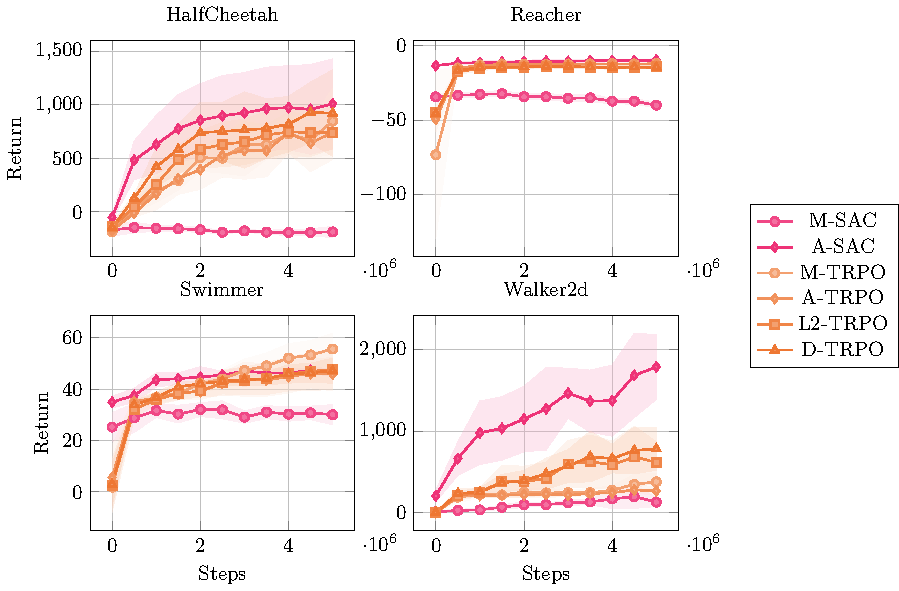
\includegraphics[labelbelief=multipledelayspendulumdtrpo]{img/thesis_plots_belief.pdf}
    \caption{Return obtained by a D-TRPO trained with delay 10 and tested on smaller delays on Pendulum.}
    \label{fig:multi_delay_pendulum_dtrpo}
\end{figure}

\begin{figure}[t]
    \centering
    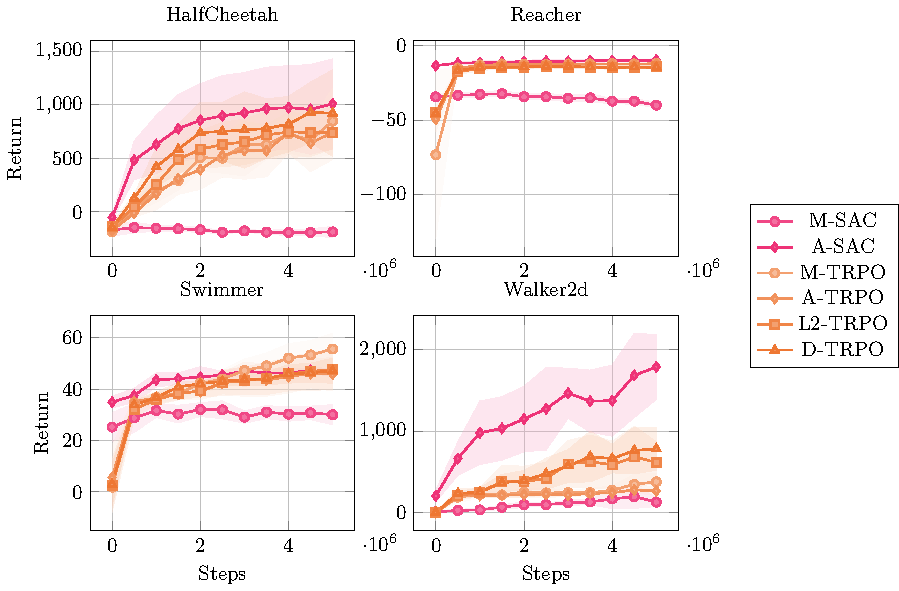
\includegraphics[labelbelief=multipledelaysmujocodtrpo]{img/thesis_plots_belief.pdf}
    \caption{Return obtained by a D-TRPO trained with delay 5 and tested on smaller delays on Mujoco environments.}
    \label{fig:multi_delay_mujoco_dtrpo}
\end{figure}

\begin{figure}[t]
    \centering
    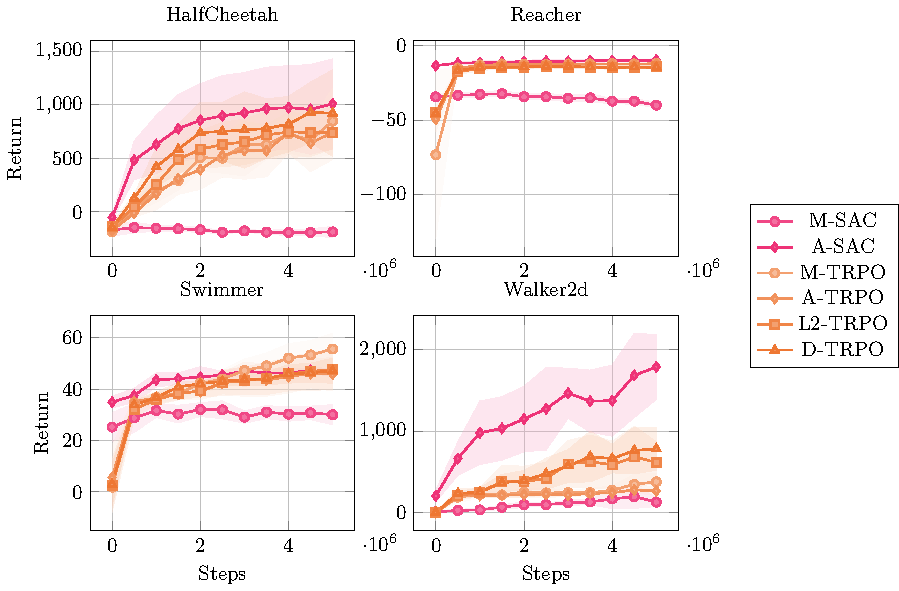
\includegraphics[labelbelief=multipledelaysmujocoltwotrpo]{img/thesis_plots_belief.pdf}
    \caption{Return obtained by an L2-TRPO trained with delay 5 and tested on smaller delays on Mujoco environments.}
    \label{fig:multi_delay_mujoco_ltrpo}
\end{figure}